
\section{Methods}\label{Sec:Method}

Based on the extensive literature review briefly presented above, two different forecasting techniques were chosen to be employed to predict households' energy consumption and production. The following criteria were considered for the selection of appropriate methods: 

\begin{enumerate}
    \item The forecasting technique had to produce deterministic (i.e., point) forecasts.
    \item The forecasting technique had to be used in existing studies about forecasting energy consumption or production.
    \item The existing study or studies using the forecasting technique had to use comparable data, i.e., recorded by smart meters, 60-min or higher resolution, recorded in multiple households, and not recorded in SMEs or other business or public buildings.
    \item The forecasting task had to be comparable to the forecasting task of this study, i.e., single consumer household (in contrast to the prediction of aggregated energy time series) and very short forecasting horizon ($\leq 24$ hours).
    \item The forecasting technique had to only take historical and calender features as input for the prediction.
    \item The forecasting technique had to produce absolutely and relative to other studies promisingly accurate predictions.
\end{enumerate}

\noindent Based on these criteria two forecasting techniques were selected for the prediction task at hand. As short-term energy forecasting techniques are commonly categorized into statistical and machine learning (or artificial intelligence) methods \citep{Bansal:2015,Diagne:2013,Gan:2017}, one method of each category was chosen: Deep recurrent neural network (DRNN) adapted from the procedure outlined by \citet{Shi:2017} and sparse autoregressive LASSO as developed and implemented by \citet{Li:2017}.%, and Kernel-Wavelet-Functional method (KWF) following the idea of \citet{Auder:2018} of using discrete wavelet transform and clustering before applying the KWF method.

Before these two methods are explained in detail, the benchmark model, that serves as a baseline for the assessment of the prediction methods, is presented next.


%%%%%%%%%%%%%%%%%%%%%%%%%%%
%%%   Benchmark model   %%%
%%%%%%%%%%%%%%%%%%%%%%%%%%%

\subsection{Benchmark model} \label{Sec:Method;Subsec:Benchmark}

Benchmark models serve as a trivial baseline to assess the relative improvement of a sophisticated model \citep{Meer:2018}. According to \citet{Pinson:2012}, a benchmark model should serve as a reference, need few computational resources to be estimated, and be model-free. A sophisticated forecasting method is only worth implementing if it can significantly outperform a trivial benchmark model \citep{Diagne:2013}. A frequent benchmark model used for deterministic forecasts is the simple persistence model \citep{Meer:2018}. This model assumes that the conditions at time $t$ persist at least up to the period of forecasting interest at time $t+h$. In energy forecasting, this na\"ive model is surprisingly well suited to forecast very short time periods of a few seconds or minutes \citep{Pinson:2012} and, thus, often harder to beat than it might seem. Here, the persistence model is defined as
%
\begin{equation} \label{Eq:naivepred}
\widehat{x}_{t+1}=x_t.
\end{equation}

There are several other benchmark models commonly used in energy load forecasting. Most of them are, in contrast to the persistence model, more sophisticated benchmarks, such as the Holt-Winters-Taylor (HTW) exponential smoothing method \citep[see, e.g.,][]{Arora:2016}. Further sophisticated benchmark models are the Vanilla benchmark \citep{hong:2010}, and the popular ARMA method \citep{Box:1990}. However, as the forecasting task at hand serves the specific use case of being an input for the bidding process in a blockchain-based local energy market, the improvement of the forecasting model over a benchmark model is of secondary importance. The task here is not so much to establish the quality of a forecasting model per se as to assess whether the available and most promising forecasting techniques can deliver accurate enough results for the use case explained above. Hence, only the persistence model will serve as a benchmark to the forecasting techniques presented next. The more relevant test of the forecasting models' accuracy will be explained in Section~\ref{Sec:Method;Subsec:Market}.



%%%%%%%%%%%%%%%%
%%%   LSTM   %%%
%%%%%%%%%%%%%%%%

\subsection{Machine learning based forecasting approach} \label{Sec:Method;Subsec:LSTM}

The first sophisticated forecasting technique that is employed to produce accurate predictions for the blockchain-based LEM is a machine learning algorithm. Even though being applied very successfully in a wide range of tasks, such as speech recognition \citep{Graves:2013} or anomaly detection in time series \citep{Malhotra:2015}, long short-term memory (LSTM) neural networks (NN) have been introduced only very recently in load forecasting studies \citep[e.g.,][]{Kong:2018,Shi:2017,Gan:2017,Chen:2018}. Compared to previous attempts using machine learning techniques, the applications of LSTM neural networks for load forecasting have been much more successful \citep{Kong:2018,Shi:2017}. This is most likely due to the high effectiveness of recurrent neural networks for sequence learning. LSTM neural networks are a advanced architecture of recurrent neural networks that are particularly well suited to learn long sequences or time series due to their ability to retain information over many time steps. The next three sections explain the basic working principles of the chosen machine learning approach and are based on \citet{chollet:2018}, \citet{Lipton:2015}, and \citet{Gan:2017}.



%%%%%%%%%%%
\subsubsection{Basic functioning of neural networks}

To understand the full advantage that LSTM recurrent neural networks have over other machine learning techniques for time series learning, it is useful to take a step back and recapitulate the basic functioning of a so-called feedforward neural network. Neural networks do not need any strong assumptions about their functional form, such as traditional time series models (e.g., ARMA). Still, they are universal approximators for finite input \citep{Hornik:1989} and, therefore, especially well suited for the prediction of such volatile time series as energy consumption or production. The most basic building blocks of any neural network are three types of layers: an input layer, one or more hidden layer(s), and an output layer. Each layer consists of one or more units (sometimes called neurons). Each unit in a layer takes in an input, applies a transformation to this input, and outputs it to the next layer (see Figure~\ref{Fig:simpleNN}). Formally, this can be written as
%
\begin{equation} \label{Eq:feedforward}
\begin{split}
    \vec{h}_{1,i}&=\phi_1\left(\vec{W}_1\vec{x}_i+\vec{b}_1\right)\\
    \vec{h}_{2,i}&=\phi_1\left(\vec{W}_2\vec{h}_{1,i}+\vec{b}_2\right)\\
    &\setbox0\hbox{=}\mathrel{\makebox[\wd0]{\hfil\vdots\hfil}}\\
    o_i&=\phi_n\left(\vec{W}_n\vec{h}_{(n-1),i}+\vec{b}_n\right)=\widehat{y}_i,
\end{split}
\end{equation}
%
where $n$ denotes a layer, $\phi_n$ is the activation function, $\vec{W}_n$ is the weight matrix, and $\vec{b}_n$ the bias vector in layer $n$. $\vec{x}_i$ is the $i^{th}$ input vector and $o_i$ the output value of the output layer which is the estimation of the true value $y_i$.
%
\begin{figure}[htbp]
    \centering
    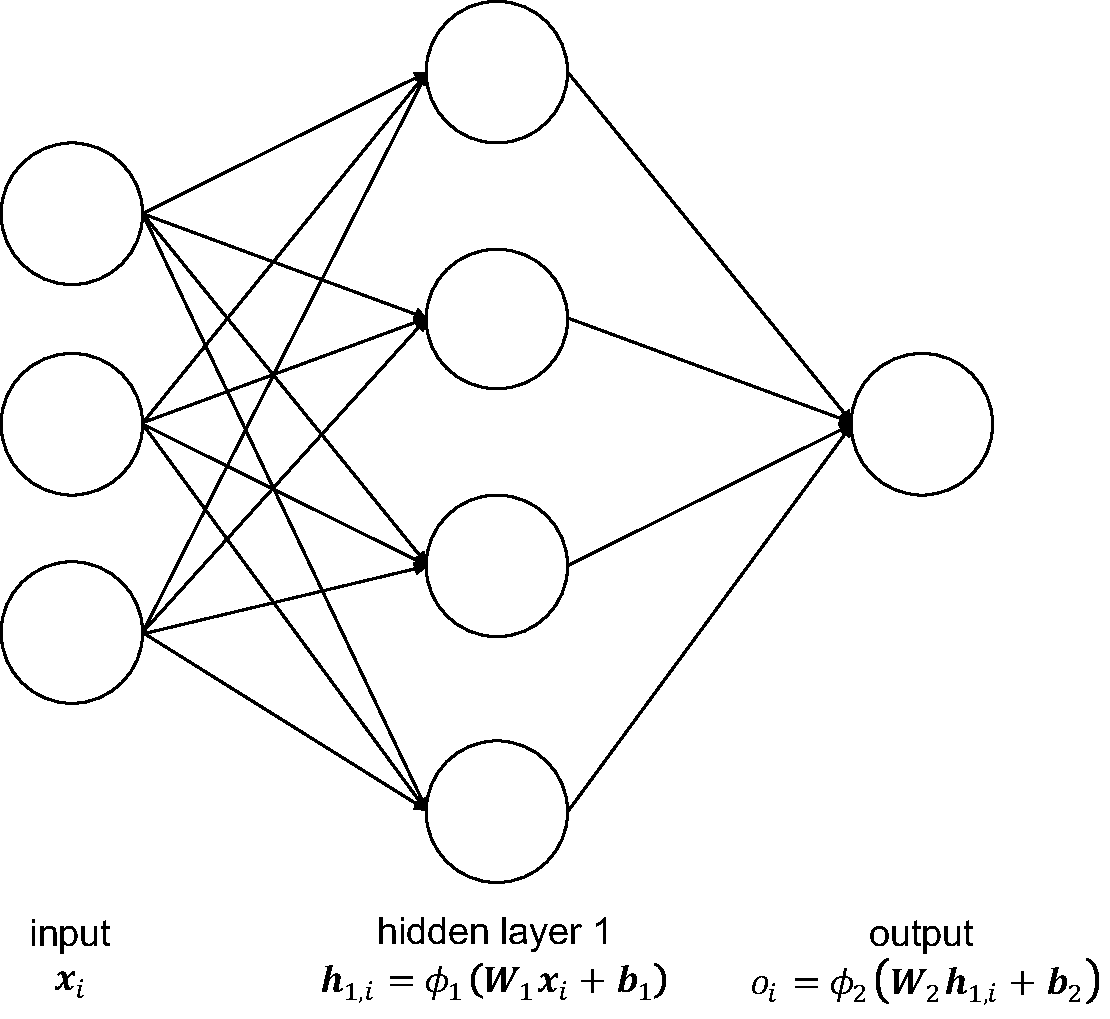
\includegraphics[scale=0.5]{thesis/figures/simpleNN.pdf}
    \caption[Schematic representation of a simple neural network]{Schematic representation of a simple neural network. Adapted from \citet{Gan:2017}.}
    \label{Fig:simpleNN}
\end{figure}

In the input layer there are as many units as there are features (i.e., variables) that serve as input for the forecasting model. The units of the input layer are connected to all units in the (first) hidden layer. The weight matrices and bias vectors in each layer are parameters that are adjusted during the training of the model. In all subsequent hidden layers, all units of one layer are connected to all units of the next layer (this is called densely connected). The last layer consists of as many units as there are output values. That is, if the forecasting model should just predict a single value, the output layer will have a single unit that takes in the weighted output values of all units of the last hidden layer, applies a transformation to these inputs and outputs a single value. The transformation that is applied to the input within each unit is called activation function and must be chosen depending on the task at hand. Especially for sequence learning, this activation function is often a hypberbolic tangent (tanh) \citep{Lipton:2015}:

\begin{equation} \label{Eq:activation}
    \phi(z)=\frac{e^z-e^{-z}}{e^z+e^{-z}}.
\end{equation}

The learning in machine learning refers in the case of neural networks to adjusting the weight matrices and bias vectors such that the best prediction is output. In supervised learning, adjusting these weights (i.e., the training of the model) is done through an algorithm that is called backpropagation which was introduced by \citet{Rumelhart:1986}. First, the weight matrices and bias vectors are randomly initialized. Then, in a first iteration, the training data is fed into the network, which outputs a prediction. This prediction is assessed with the help of a loss function that quantifies the distance between the prediction and the true value. A commonly used loss function is the mean absolute error:
%
\begin{equation} \label{Eq:lossMAE}
    L\left(y, \widehat{y}\right)=\text{MAE}=\frac{1}{N}\sum_{i=1}^N\left|\widehat{y}_i-y_i\right|
\end{equation}
%
The simplest method to optimize the model parameters is to compute the derivative of the loss function with respect to each parameter in the model and change each parameters in a fixed-size step in the direction of the negative gradient \citep{Graves:2013}. This method is called gradient descent. Thereby the prediction error is ``backpropagated" through the network to update the parameters. This is repeated in each iteration until the model converges to a value of the loss function that cannot be further improved.



%%%%%%%%%%%
\subsubsection{Recurrent neural networks}

Unfortunately, feedforward neural networks are not particularly well-suited for time series learning \citep{chollet:2018}. This is because simple neural networks, such as the one described above, do not have an internal state that could retain a memory of previously processed input. That is, to learn a sequence or time series, a feedforward neural network would always need the complete time series as a single input. It cannot retain a memory of something learned in a previous chunk of the time series to apply it to the next chunk that is fed into the model. This problem is tackled by recurrent neural networks.

Recurrent neural networks still consist of the basic building blocks of units and layers. However, the units do not just feed forward the transformed input as output but have a recurrent connection that feeds an internal state back into the unit as input (see Figure~\ref{Fig:RNNunit}). Thereby, a RNN unit loops over individual elements of an input sequence, instead of processing the whole sequence in a single step. This means, the RNN unit applies the transformation to the first element of the input sequence and combines it with its internal state. This introduces the notion of time into neural networks. Formally, this can be written as
%
\begin{equation} \label{Eq:RNN}
\begin{split}
    \vec{h}_{1,t}&=\phi_1\left(\vec{W}_1^{(i)}\vec{x}_t+\vec{W}^{(r)}_1\vec{h}_{1,(t-1)}+\vec{b}_1\right)\\
    \vec{h}_{2,t}&=\phi_2\left(\vec{W}_2^{(i)}\vec{h}_{1,t}+\vec{W}^{(r)}_2\vec{h}_{2,(t-1)}+\vec{b}_2\right)\\
    &\setbox0\hbox{=}\mathrel{\makebox[\wd0]{\hfil\vdots\hfil}}\\
    o_t&=\phi_n\left(\vec{W}_n^{(i)}\vec{h}_{(n-1),t}+\vec{b}_n\right)=\widehat{y}_t,
\end{split}
\end{equation}
%
where $n$ denotes a layer, $\phi_n$ is the activation function, $\vec{W}_n^{(i)}$ is the weight matrix for the input, $\vec{W}_n^{(r)}$ is the weight matrix for the recurrent input (i.e., the output of layer $n$ in the previous time step), and $\vec{b}_n$ the bias vector in layer $n$. $\vec{x}_t$ is the input vector at time $t$ and $o_t$ the output value of the output layer which is the estimation of the true value $y_t$. Note that the output layer has no recurrent units but is the same as in a simple feed forward network.
%
\begin{figure}[htbp]
    \centering
    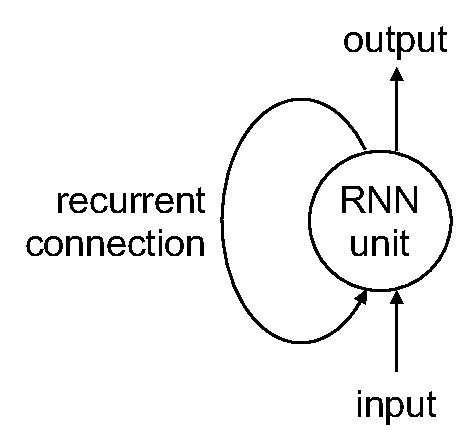
\includegraphics[scale=0.5]{thesis/figures/RNNunit.pdf}
    \caption[Schematic representation of a RNN unit]{Schematic representation of a RNN unit. Adapted from \citet{chollet:2018}.}
    \label{Fig:RNNunit}
\end{figure}

The cyclical structure of an RNN unit can be unrolled across time (see Figure~\ref{Fig:RNNunfolded}). This illustrates that a RNN is basically a simple neural network that has one layer for each time step that has to be processed per input. This notion of an unfolded RNN also reveals, that a RNN is still trainable through backpropagation. The backpropagation just has to happen across all time steps. This is called backpropagation through time (BPTT) and was introduced by \citet{Werbos:1990}. Theoretically, this feedback structure enables RNN to retain information about sequence elements that have been processed many steps before the current step and use it for the prediction of the current step. However, in practice the vanishing gradient problem occurs\footnote{For more details on the vanishing gradient problem see, e.g., \citet{Bengio:1994}}. This problem makes RNNs for very long sequences basically untrainable.
%
\begin{figure}[htbp]
    \centering
    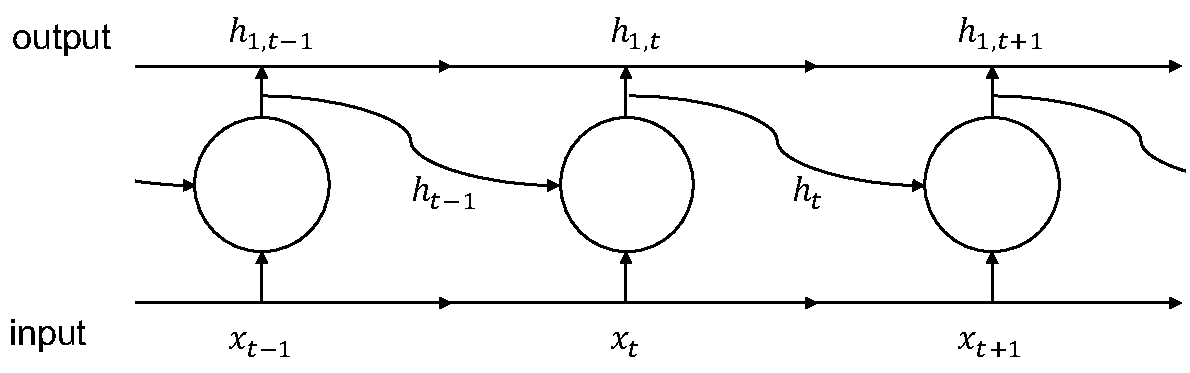
\includegraphics[scale=0.6]{thesis/figures/RNNunfolded.pdf}
    \caption[Schematic representation of an unfolded RNN unit]{Schematic representation of an unfolded RNN unit. Adapted from \citet{chollet:2018}.}
    \label{Fig:RNNunfolded}
\end{figure}



%%%%%%%%%%%
\subsubsection{Long short-term memory units}

To overcome the vanishing gradient problem, \citet{Hochreiter:1997} developed LSTM units. LSTM units extend RNN units by an additional state. This state can retain information for as long as needed. In which step this additional state is updated and in which state the information it retains is used in the transformation of the input is controlled by three so-called gates\footnote{In their original specification, \citet{Hochreiter:1997} included only two gates. However, as this LSTM specification was still prone to the vanishing gradient problem under some circumstances, \citet{Gers:2000} extended it by a third gate.}. These three gates again have the form of a simple RNN cell. Formally, the gates can be written as (following the notation of \citet{Lipton:2015}\footnote{\cites{Lipton:2015} notation uses $h_{t-1}$ instead of $s_{t-1}$. The notation used here ($s_{t-1}$) accounts for the modern LSTM architecture with peephole connections. For more information see \cite{Gers:2002}.})
%
\begin{equation} \label{Eq:LSTMgates}
\begin{split}
    \vec{i}_t&=\sigma\left(\vec{W}^{(ix)}\vec{x}_t+\vec{W}^{(is)}\vec{s}_{t-1}+\vec{b_i}\right)\\
    \vec{f}_t&=\sigma\left(\vec{W}^{(fx)}\vec{x}_t+\vec{W}^{(fs)}\vec{s}_{t-1}+\vec{b_f}\right)\\
    \vec{o}_t&=\sigma\left(\vec{W}^{(ox)}\vec{x}_t+\vec{W}^{(os)}\vec{s}_{t-1}+\vec{b_o}\right),
\end{split}   
\end{equation}
%
where $\sigma$ is the sigmoid activation function $\sigma(z)=\frac{1}{1+e^{-z}}$, $W$ denotes the weight matrices that are intuitively labeled ($ix$ for the weight matrix of gate $i_t$ multiplied with the input $x_t$ etc.), and $b$ denotes the bias vectors.\footnote{Sometimes, the gates are titled input, output, and forget gate. However, as \citet{chollet:2018} put it:
\vspace{0.75\dimexpr-\topsep-\partopsep}
\begin{quote}
    ``[T]hese interpretations don’t mean much, because what these [gates] actually do is determined by the contents of the weights parameterizing them; and the weights are learned in an end-to-end fashion, starting over with each training round, making it impossible to credit this or that operation with a specific purpose" (p. 193).
\end{quote}\vspace{\dimexpr-\topsep-\partopsep}
}

Again following the notation of \citet{Lipton:2015}, the full algorithm of a LSTM unit is given by the three gates specified above, the input node
%
\begin{equation} \label{Eq:LSTMinput}
    \vec{g}_t=\sigma\left(\vec{W}^{(gx)}\vec{x}_t+\vec{W}^{(gh)}\vec{h}_{t-1}+\vec{b_g}\right),
\end{equation}
%
the internal state of the LSTM unit at time step $t$
%
\begin{equation} \label{Eq:LSTMstate}
    \vec{s}_t=\vec{g}_t\odot\vec{i}_t+\vec{s}_{t-1}\odot\vec{f}_t,
\end{equation}
%
where $\odot$ is pointwise multiplication, and the output at time step $t$
%
\begin{equation} \label{Eq:LSTMoutput}
    \vec{h}_t=\phi\left(\vec{s}_t\right)\odot\vec{o}_t.
\end{equation}
%
The internal structure of a LSTM cell is further clarified by Figure~\ref{Fig:LSTMunit}. For an intuitive but more detailed explanation of LSTM neural networks see \citet[][Ch. 6.2]{chollet:2018}
%
\begin{figure}[htbp]
    \centering
    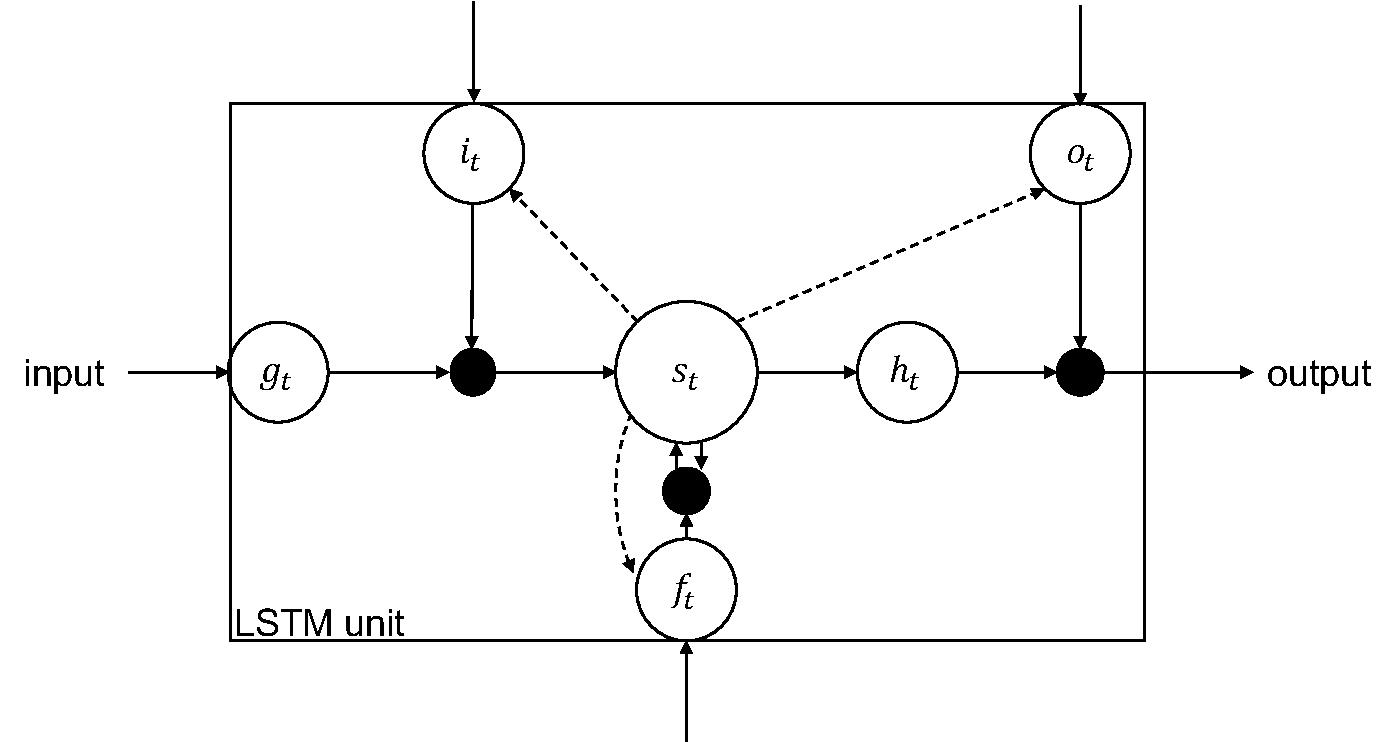
\includegraphics[scale=0.5]{thesis/figures/LSTMunit.pdf}
    \caption[Schematic representation of a LSTM unit]{Schematic representation of a LSTM unit. Adapted from \citet{Graves:2012}. The filled in circles represent the pointwise multiplication operation denoted by $\odot$ in Equation~\ref{Eq:LSTMstate} and~\ref{Eq:LSTMoutput}.}
    \label{Fig:LSTMunit}
\end{figure}

To summarize, all neural networks use the basic building blocks of units that form input, hidden, and output layers. The training process of neural networks involves updating the parameters (weights and biases) of the model based on the gradient descent of a loss function that quantifies the accuracy of a prediction compared to true values. RNN enables the neural network to process individual elements of a sequence or time series sequentially and still use information that was obtained in previous time steps for the current transformation of the input. LSTM RNN is an extension of simple RNN which has the advantage of being able to retain a state over multiple time steps and solves the vanishing gradient problem through the introduction of an additional internal state $\vec{s}_t$. By this, LSTM RNN are capable of learning highly complex, non-linear relationships in time series data which makes them a promising forecasting technique to predict households' very short-term energy consumption and production.



%%%%%%%%%%%
\subsubsection{Implementation of LSTM RNN}

The specific LTSM RNN approach adopted in this study is based on the procedure employed by \citet{Shi:2017} to forecast individual households' energy consumption. However, according to the relevant use case in this study, model training and predictions were performed using only the data of individual households. That means, a LSTM recurring neural network was trained for each household individually using only the households historic consumption patterns and calender features. This differs from \cites{Shi:2017} implementation, that used pooled consumption data of multiple households. Specifically, seven weeks of past consumption, an indicator for weekends, and an indicator for Germany-wide holidays were used as input for the neural network in the present study. The target values were single consumption values in 15-minute aggregation. Take the following example as illustration: The consumption values in 3-minute intervals from 13.11.2017 13:00 until 20.11.2017 13:00 and zero/one-indicators for weekends and holidays (i.e., 3 $\times$ 3360 data points) are fed into the neural network. The model then produces a single output value that estimates the household's energy consumption in kWh from 20.11.2017 13:00 until 20.11.2017 13:15.

A neural network is defined by several so-called hyperparameters: The number and type of layers, the number of hidden units within each layer, the activation functions used within each unit, dropout rates for the recurrent transformation, and dropout rates for the transformation of the input. These hyperparameters must be chosen particularly for the task at hand and their influence on the model performance is difficult to foresee. For this reason, parameter tuning was employed to find a relatively well working combination of hyperparameter values. Unfortunately, hyperparameter tuning is computationally very resource intensive as for each hyperparameter combination, the model must be fully trained to asses the model performance. Hence, not all possible or sensible combinations of hyperparameters could be assessed. Instead, a random sample of different hyperparameter combinations was chosen and the resulting model configurations trained and evaluated on a randomly chosen data set.

Table~\ref{Tab:LSTMHyperparameters} presents the hyperparameters that were tuned and their respective value ranges. The tuning was done individually for each layer. First layer 1 hyperparameters were tuned. The best found hyperparameter combination was then fixed for layer 1 and the parameters for layer 2 were tuned. This was repeated for layer 3. Optimally, all hyperparameters should be tuned simultaneously. However, due to computational constraints, that was not possible here and, thus, the described, second-best option chosen. As the hyperparameter values specified in Table~\ref{Tab:LSTMHyperparameters} for layer 1 alone result in 81 possible hyperparameter combinations, only samples of these combinations were taken, the resulting models trained and compared. In total, 16 models with one layer, 13 models with two layers and 13 models with 3 layers were tuned. The model tuning was conducted on the Machine Learning (ML) Engine of the Google Cloud Platform. The job was submitted to The ML Engine via Google Cloud SDK and the R package \texttt{cloudml}. The model training was conducted on four Tesla P100 GPUs. The necessary credits to pay for the hardware resources were granted by Google as part of their Google Cloud Platform Free Tier program\footnote{For further details see \url{https://cloud.google.com/free} (last accessed 01.10.2018).}.

\begin{table}[htbp]
    \begin{center}
        {\footnotesize
        \begin{tabular}{l|lcccc}
        \hline \hline
        & \multirow{2}{3em}{hyperparameter} & possible & possible     & sampling & \# of assessed \\
        &                                   & values   & combinations & rate     & combinations   \\
        \hline
                \multirow{4}{3em}{layer 1}  & batch size        & \{128, 64, 32\} & \multirow{4}{1em}{81} & \multirow{4}{1em}{0.2} & \multirow{4}{1em}{16} \\
                                            & hidden units      & \{128, 64, 32\} & & &\\
                                            & recurrent dropout & \{0, 0.2, 0.4\} & & & \\
                                            & dropout           & \{0, 0.2, 0.4\} & & & \\[0.2cm]
                                            & hidden units      & \{128, 64, 32\} & & & \\
                layer 2                     & recurrent dropout & \{0, 0.2, 0.4\} & 26 & 0.5 & 13 \\
                                            & dropout           & \{0, 0.2, 0.4\} & \\[0.2cm]
                                            & hidden units      & \{128, 64, 32\} & \\
                layer 3                     & recurrent dropout & \{0, 0.2, 0.4\} & 26 & 0.5 & 13 \\
                                            & dropout           & \{0, 0.2, 0.4\} & \\
            \hline \hline
        \end{tabular}}
    \end{center}
    \caption[Hyperparameters tuned for optimal LSTM RNN model specification]{The hyperparameters and their possible values that were tuned for an optimal LSTM RNN model specification.}
    \label{Tab:LSTMHyperparameters}
\end{table}

As it turned out, a deeper model architecture of multiple layers did not increase the model performance enough to justify the greatly increased computing time for model training introduced by the much higher number of model parameters that would have to be trained\footnote{A one layer, 32 hidden units LSTM RNN with one output unit has 4,641 trainable parameters while a two layer, 32 hidden units each LSTM RNN with one output unit has already 12,961 trainable parameters.}. Therefore, a model of the following specification was used for the prediction of a single energy consumption value for the next 15 minutes:

\indent\textit{layers: $1$\\
\indent hidden units: $32$\\
\indent dropout rate: $0$\\
\indent recurrent dropout rate: $0$\\
\indent batch size: $32$\\
\indent number of input data points: $3360$\\
\indent number of training samples\footnote{Each sample consists of an array of the dimensions batch size $\times$ input data points $\times$ input features, i.e., 32$\times$3360$\times$3. Thus, the number of training samples has to be multiplied by the batch size and the number of data points that are aggregated for each prediction (i.e., 5) to get the total length of data points covered in the training process: $700*32*5=112000$ data points. This is equivalent to the time period from 01.01.2017 00:00 to 2017-08-22 09:03}: $700$ \\
\indent number of validation samples: $96$}

The general procedure of model training, model assessment and prediction generation is shown as pseudo code in Procedure~\ref{Alg:LSTMimplementation}. The first step of setting the parameter tuple is done globally for all household data sets based on the results of the hyperparameter tuning. Thereafter, the same procedure is repeated for each data set.

First, the consumption data time series is loaded, target values are generated, and the input data is transformed. The transformation consists of normalizing the log-values of the consumption per 3-minute interval between 0 an 1. A graph showing the distribution of energy consumption before and after the transformation exemplary for one data set is shown in Appendix~\hyperlink{AppA3:Figures:transform}{A3}. This ensures fast convergence of the model training process. The data batches for the model training and the cross-validation are served to the training algorithm by so-called generator functions. The generator functions are called by the training algorithm and supply samples of data from the input time series infinitely. The number of training and validation steps that are necessary for the model to see the complete input time series is controlled by the training algorithm.
%
\begin{algorithm}[htbp]
\floatname{algorithm}{Procedure}
\caption{Supervised learning of LSTM neural network and prediction.}\label{Alg:LSTMimplementation}

\begin{algorithmic}[1]
\State{Set parameter tuple $<l, u, b, d>$: number of layers $l \subseteq L$, number of hidden LSTM-units $u \subseteq U$, batch size $b \subseteq B$, and dropout rate $d \subseteq D$.}
\State{Initiate prediction matrix $P$ and list for error measures $\Theta$.}
\For{Household $i$ in data set pool $I$}
    \State{Load data set $\Psi_i$ of consumer $i$.}
    \State{Generate target values $\vec{y}$ by aggregating consumption data to 15-min intervals.}
    \State{Transform consumption time series in data set $\Psi_i$ and add calender features.}
    \State{Set up training and validation data generators according to parameter tuple $<b, d>$.}
    \State{Split data set $\Psi_i$ into training data set $\Psi_{i,tr}$ and testing data set $\Psi_{i,ts}$.}
    \State{Build LSTM RNN $\zeta_i$ on Tensorflow with network size $(l, h)$.}
    \Repeat
    \indent\State{\textbf{At} $k^{th}$ epoch \textbf{do}:}
        \State{\multiline{%
        Train LSTM RNN $\zeta_i$ with data batches $\varphi_{train} \subseteq \Psi_{i,tr}$ supplied by training data generator.}}
        \State{\multiline{%
        Evaluate performance with mean absolute error $\Lambda_k$ on cross-validation data batches $\varphi_{val} \subseteq \Psi_{i,tr}$ supplied by validation data generator.}}
    \Until{$\Lambda_{k-1}-\Lambda_{k}<0.001$ for the last 3 epochs.}
    \State{Save trained LSTM RNN $\zeta_i$.}
    \State{Set up testing data generator according to tuple $<b, d>$.}
    \State{\multiline{%
    Generate predictions $\vec{\widehat{y}_i}$ with batches $\varphi_{ts} \subseteq \Psi_{i,ts}$ fed by testing data generator into LSTM RNN $\zeta_i$.}}
    \State{Calculate error measures $\Theta_i$ to assess performance of $X_i$.}
    \State{Write prediction vector $\vec{\widehat{y}_i}$ into column $i$ of matrix $P$.}
\EndFor
\State{Save matrix $P$.}
\State{\textbf{End.}}
\end{algorithmic}

\end{algorithm}
%
Second, the LSTM RNN is compiled and trained. This is done with Keras which is a neural network API written in Python. It can employ several machine learning back-ends that are based on computational graphs. The most commonly known and very well-developed back-end is TensorFlow by Google which is an open source software that enables parallel GPU-based numerical computations\footnote{For more details on tensors and TensorFlow see \citet{Abadi:2017, Goldsborough:2016}}. The \texttt{keras} R package (v2.2.0.9), which this study used, is a wrapper of the Python library and is maintained by \citet{chollet:2017kerasR}. The package was used with RStudio v1.1.453 and TensorFlow 1.11.0 as back-end. The model training and prediction for each household was performed on a Windows Server 2012 with 12 cores and 24 logical processors of Intel Xeon 3.4 GHz CPUs\footnote{The computing resources were kindly provided by the Humboldt Lab for Empirical and Quantitative Research (LEQR) at the School of Business and Economics, Humboldt-University Berlin.}. The model training is done in a differing number of epochs as early stopping was employed. That means, once the mean absolute error on the validation data did not decrease by more than 0.001 in three consecutive epochs, the training process is stopped (see line 14 in Procedure~\ref{Alg:LSTMimplementation}). Early stopping is a common and well-suited approach to prevent overfitting \citep{chollet:2018}.

Finally, the trained model was used to generate predictions on the test set that comprises data from 01.10.2017 00:00 to 01.01.2018 00:00 (i.e., 44,180 data points). As the prediction was made in 15-minute intervals, in total, 8,836 data points were predicted. Using the error measures described in Section~\ref{Sec:Method;Subsec:Error}, the model performance was assessed. Additionally, the predictions for all data sets were saved for the evaluation of the prediction in the context of the market mechanism implemented in a smart contract by \citet{Mengelkamp:2018a}.

%%%%%%%%%%%%%%%%%
%%%   LASSO   %%%
%%%%%%%%%%%%%%%%%

\subsection{Statistical method based forecasting approach} \label{Sec:Method;Subsec:LASSO}

To complement the machine learning approach of LSTM neural networks with a statistical approach, a second, regression-based method was chosen. For this purpose, the sparse autoregressive LASSO algorithm proposed by \citet{Li:2017} seemed most suitable. Statistical methods have the advantage of much lower model complexity compared to neural networks which makes them computationally much less resource intensive. Additionally, a LASSO-based approach as employed by \citet{Li:2017} maintains the easy interpretability of linear methods.



%%%%%%%%%%%
\subsubsection{Sparse autoregressive LASSO}

The approach proposed by \citet{Li:2017} is based on a linear autoregressive model:
%
\begin{equation} \label{Eq:ARmodel}
    y_{t+1}=\beta_0+\sum_{i=0}^I\beta_iy_{t-i}+\varepsilon_t,
\end{equation}
%
where the future demand $y_{t+1}$ depends linearly only historical data $y_{t-i}$ plus a random Gaussian noise $\varepsilon_t$, with $\beta_i$ being the coefficient for lag-order $i$. In the following, vector $\left[y_t, y_{t-1}, \dots, y_{t-I}\right]^T$ is written as $\vec{x_t}$. Using the model in Equation~\ref{Eq:ARmodel} for prediction is achieved by estimating the vector $\widehat{\beta}$ such that the sum of squared errors is minimal. However, as the OLS estimator
%
\begin{equation} \label{Eq:betaOLS}
    \widehat{\vec{\beta}}_{\text{OLS}}=\argmin_{\vec{\beta}}\left\lVert(\vec{y}-\vec{X}\vec{\beta}\right\rVert^2_2
\end{equation}
%
minimizes the sum of squared error within the data used to estimate $\widehat{\vec{\beta}}_{\text{OLS}}$, it is very likely to overfit the data and to have a very poor prediction accuracy on new data.

This risk of model overfitting can be mitigated by including only lag-orders of the historical data that are relevant for the estimation of $y_{t+1}$ and thereby reducing the number of regressors. Thus, \citet{Li:2017} use least absolute shrinkage and selection to find a sparse autoregressive model which generalizes better to new data. Formally, the LASSO estimator can be written as
%
\begin{equation} \label{Eq:betaLASSO}
    \widehat{\vec{\beta}}_{\text{LASSO}}=\argmin_{\vec{\beta}}\frac{1}{2}\left\lVert(\vec{y}-\vec{X}\vec{\beta}\right\rVert^2_2+\lambda\left\lVert\vec{\beta}\right\rVert_1,
\end{equation}
%
where $\lambda$ is a parameter that controls the level of sparsity in the model, i.e., the number of lag-orders that are included to predict $y_{t+1}$. This model specification selects the best recurrent pattern in the energy time series by shrinking coefficients of irrelevant lag-orders to zero and thereby improves the generalizability of the prediction model.



%%%%%%%%%%%
\subsubsection{Implementation of sparse autoregressive LASSO}

The sparse autoregressive LASSO approach was implemented using the R package \texttt{glmnet} \citep{Friedman:2010}. Again, as for the LSTM RNN approach, model training and prediction were performed for every household individually. Following \cites{Li:2017} procedure, only historical consumption values were used as predictors. Specifically, seven weeks of lagged consumption values served as input to the LASSO model. The response vector consisted of single consumption values in 15-minute aggregation. The same example as above is presented for illustration of the prediction task: The consumption values in 3-minute intervals from 13.11.2017 13:00 until 20.11.2017 13:00 (i.e., 3360 data points) are available to the model for prediction. 
Based on the training data, the model chooses the lagged values with the highest predictive power and makes a linear estimation of a single value for the household's energy consumption in kWh from 20.11.2017 13:00 until 20.11.2017 13:15.

The \texttt{glmnet} package used for this task fits a generalized linear model with the  elastic-net penalty
%
\begin{equation} \label{Eq:elasticnetpenalty}
    \lambda\left[(1-\alpha)\left\lVert\vec{\beta}\right\rVert^2_2/2 + \alpha \left\lVert\vec{\beta}\right\rVert_1\right],
\end{equation}
%
where $\alpha=1$ to perform LASSO. Hence, the penalty term here is $\lambda\left\lVert\vec{\beta}\right\rVert_1$. The parameter $\lambda$ has to be tuned. This can be done using the package's cross-validation function with parallel computing. As a linear autoregressive model had to be fitted, the Gaussian family option of the package was chosen. The objective function of the Gaussian family LASSO model is
%
\begin{equation} \label{Eq:glmnetobjfun}
    \min_{(\beta_0, \vec{\beta)}}\frac{1}{2N} \sum_{i=1}^N (y_i -\beta_0-x_i^T\vec{\beta})^2+\lambda\left\lVert\vec{\beta}\right\rVert_1,
\end{equation}
%
where $\lambda \geq 0$ is the tuning parameter that controls by how much the number of coefficients is penalized. The objective function is solved by applying coordinate descent \citep[for more details see][]{Friedman:2010}.

As the LASSO model requires a predictor matrix, the time series of each household is split in sequences of length $n=3360$ with 5 data points skipped in between. The skip accounts for the fact, that the response vector is comprised of 15-minute interval consumption values (i.e., five 3-minute consumption values). The detailed description of the model estimation and prediction is presented in Procedure~\ref{Alg:LASSOimplementation}.
%
\begin{algorithm}[htbp]
\floatname{algorithm}{Procedure}
\caption{Cross-validated selection of $\lambda$ for LASSO and prediction.} \label{Alg:LASSOimplementation}

\begin{algorithmic}[1]
\State{Initiate prediction matrix $P$ and list for error measures $\Theta$.}
\For{Household $i$ in data set pool $I$}
    \State{Load data set $\Psi_i$ of consumer $i$.}
    \State{Generate target values $\vec{y}$ by aggregating consumption data to 15-min intervals.}
    \State{Split data set $\Psi_i$ into training data set $\Psi_{i,tr}$ and testing data set $\Psi_{i,ts}$.}
    \State{\multiline{%
    Generate predictor matrix $M_{tr}$ by slicing consumption time series from $\Psi_{i,tr}$ with sliding window.}}
    \State{Generate sequence of $\lambda$-values $\{l_s\}_{s=1}^L$.}
    \State{Set number of cross-validation (CV) folds $K$.}
    \State{Split predictor matrix $M_{tr}$ into $K$ folds.}
    \For{$k$ in $K$}
        \State{Select fold $k$ as CV testing set and folds $j\neq k$ as CV training set.}
        \For{each $l_s$ in $\{l_s\}_{s=1}^L$}
            \State{Compute vector $\widehat{\vec{\beta}}_{k,l_s}$ on CV training set.}
            \State{Compute mean absolute error $\Lambda_{k,l_s}$ on CV testing set.}
        \EndFor
    \EndFor
    \State{For each $\widehat{\vec{\beta}}_{k,l_s}$ calculate average mean absolute error $\bar{\Lambda}_s$ across the $K$ folds.}
    \State{\multiline{%
    Select cross-validated $\lambda$-value $l_s^{CV}$ with the highest regularization (i.e., lowest number of non-zero $\beta$-coefficients) within one standard deviation of the minimum $\bar{\Lambda}_s$.}}
    \State{Compute $\widehat{\vec{\beta}}_{l_s^{CV}}$ on complete predictor matrix $M_{tr}$.}
    \State{\multiline{%
    Generate predictor matrix $M_{ts}$ by slicing consumption time series from $\Psi_{i,ts}$ with sliding window.}}
    \State{\multiline{%
    Generate predictions $\vec{\widehat{y}_i}$ from predictor matrix $M_{ts}$ and coefficients $\widehat{\vec{\beta}}_{l_s^{CV}}$.}}
    \State{Calculate error measures $\Theta_i$ to assess performance.}
    \State{Write prediction vector $\vec{\widehat{y}_i}$ into column $i$ of matrix $P$.}
\EndFor
\State{Save matrix $P$.}
\State{\textbf{End.}}
\end{algorithmic}

\end{algorithm}
%

After generating the predictor matrix for the model estimation, the optimal $\lambda$ is found in a K-fold cross-validation. Here, $K$ is set to 10. The sequence of $\lambda$-values that is tested in the cross-validation is by default of length $L=100$. However, the \texttt{glmnet} algorithm uses early-stopping to reduce computing times if the percent of null deviance explained by the model with a certain $\lambda$ does not change sufficiently from one to the next $\lambda$-value. According to \citet{Friedman:2010} the sequence of $\lambda$-values is constructed by calculating the minimum lambda value as a fraction of the maximum lambda value ($\lambda_{min}=\varepsilon\lambda_{max}$, where $\lambda_{max}$ is such that all $\beta$-coefficients are set equal to zero) and moving along the log-scale from $\lambda_{max}$ to $\lambda_{min}$ in $L$ steps. The cross-validation procedure identifies the biggest $\lambda$ that is still within one standard deviation of the $\lambda$ with the lowest mean absolute error. The final coefficients for each household are then computed by solving Equation~\ref{Eq:betaLASSO} for the complete predictor matrix.

Thereafter, the predictions are made on the testing data. For this, again, the time series is sliced according to the sliding window of length $n=3360$ skipping 5 data points and written into a predictor matrix. This matrix comprises data from 01.10.2017 00:00 to 01.01.2018 00:00 (i.e., 8836 cases of 3360 lagged values), resulting again in 8836 predicted values as in the case of the LSTM neural network described above. The predictions on all data sets were assessed using the error measures described in Section~\ref{Sec:Method;Subsec:Error} and saved for the evaluation of the prediction in the context of the market mechanism implemented in a smart contract by \citet{Mengelkamp:2018a}.


%%%%%%%%%%%%%%%%%%%%%%%%%%
%%%   Error measures   %%%
%%%%%%%%%%%%%%%%%%%%%%%%%%

\subsection{Error measures} \label{Sec:Method;Subsec:Error}

Error measures play an essential role in any prediction task. Also called performance metrics, these measures are used to quantify the accuracy of the prediction generated by a forecasting model \citep{zor:2017}. Without assessing the prediction accuracy through error measures, it is impossible to quantify whether the proposed forecasting technique is an improvement compared to the benchmark models \citep{Meer:2018}. Moreover, error measures are used by supervised machine learning algorithms to assess the prediction accuracy in cross-validation and to accordingly adjust their parameters.

However, there is a wide variaty of error measures available and actively used in the research of energy forecasting. \citet{zor:2017} reviewed the energy forecasting literature published in 2017 and found eight different error measures that were used to assess the forecasting accuracy. Among those, mean absolute percentage error was used in 83~\% of the studies, with mean absolute error and root mean squared error coming third and second with 32 and 31~\% respectively. As these results suggest, there is a lack of standardization in the field of energy forecasting regarding the usage of the various available error measures \citep{Meer:2018}. This is aggravated by the fact, that different error measures are appropriate in different use cases and cannot be generally applied without careful consideration. Therefore, the following section introduces the error measures used in the research at hand and discusses their advantages and disadvantages. Following the suggestion of \citet{Hoff:2013} several performance metrics will be used to evaluate the quality of the forecast models. The choice of performance metrics is mostly guided by the compilation provided by \citet{Meer:2018}.


%%%%%%%%%%%
\subsubsection{MAE and RMSE}

Error measures can be classified into representing absolute or percentage errors \citep{Hoff:2013}. Absolute error measures are, for example, mean absolute error (MAE) and root mean squared error (RMSE). Both are quite popular as performance metrics for energy forecasts \citep{zor:2017}. Absolute error measures can be formulated in terms of a vector function 
%
\begin{equation} \label{Eq:vectorfunction}
    E=F\left(\vec{f}, \vec{x}\right),
\end{equation}

\noindent where $\vec{f}$ and $\vec{x}$ are the forecasted and actual data vectors respectively \citep{Haben:2014}. The metric $F$ is then the absolute p-norm,
%
\begin{equation} \label{Eq:pnorm}
    E_p=\left\lVert\vec{f}-\vec{x}\right\rVert_p=\biggl(\sum_{t=1}^N \left|f_t-x_t\right|^p\biggr)^{1/p},
\end{equation}

\noindent for $p\geq1$ \citep[][p. 52]{golub:2012}. The MAE belongs to this type of error and is defined as the average of the absolute differences between the predicted and true values \citep{Hoff:2013}:
%
\begin{equation} \label{Eq:MAE}
\text{MAE}=\frac{1}{N}\sum_{t=1}^N\left|\widehat{x}_t-x_t\right|,    
\end{equation}

\noindent where N is the length of the forecasted time series, $\widehat{x}_t$ the forecasted value and $x_t$ the observed value. This is equivalent to Equation~\ref{Eq:pnorm} with $p=1$. Similar to the MAE and also of the p-norm type of error measure is the RMSE. Instead of summing up the \textit{absolute} differences, the RMSE is defined as the square root of the average \textit{squared} differences (which is equivalent to $p=2$ in Equation~\ref{Eq:pnorm}):
%
\begin{equation} \label{Eq:RMSE}
\text{RMSE}=\sqrt{\frac{1}{N}\sum_{t=1}^N\left(\widehat{x}_t-x_t\right)^2}.
\end{equation}

\noindent RMSE, thus, puts more weight on large deviations between forecast and observation than MAE \citep{Meer:2018}. Therefore, RMSE is more suitable in the presence of a lot of noise, as it does not mask a small amount of large errors in the presence of a majority of small errors as the MAE does \citep{Zhang:2015}. One disadvantage of these measures is that they are not scale independent. This makes them unsuitable to compare the prediction accuracy of a forecasting model on different time series. However, they are suitable for cross-validation in machine learning algorithms and for the comparison of sophisticated forecasting techniques with benchmark models on the same time series. Moreover, they do not rely on denominator-related assumptions -- as percentage error measures do -- which makes them more robust \citep{Hoff:2013}.


%%%%%%%%%%%
\subsubsection{MAPE and NRMSE}

Even though MAE and RMSE are widely used, they are not useful to compare the forecast accuracy across different time series as they are not scale independent \citep{Meer:2018}. Therefore, it is reasonable to complement them with percentage error measures which are normalized by a denominator. However, depending on the application, there may be several denominators that could be used, each coming with certain advantages and disadvantages. \citet{Hoff:2013}, for example, found that the choice of the denominator influences the calculated error results of solar irradiance forecasts substantially. Generally, the denominator may fall into one of two categories: (1) It is a fixed single number that is representative of the time series to be forecasted (e.g., the maximum value of the time series, the average value of the time series or the maximum capacity of the electrical system under consideration) as proposed by \citet{Hoff:2013} and agreed on by \citet{Meer:2018}. (2) The denominator can be different for every pair of true and predicted value (i.e., the true value is used as denominator for each pair of true and predicted values) as defined by \citet{Hyndman:2006} and used by \citet{xie:2018}, for example. 

Investigating forecasting error measures for PV power plants, \citet{Hoff:2013} conclude that normalizing the MAE by the average output of a PV power plant is most desirable to compute the MAPE. However, as \citet{Meer:2018} did not find any literature supporting this for consumption forecasting, the MAPE and NRMSE normalised by the true value will be used here. Hence, they are defined as
%
\begin{equation} \label{Eq:MAPE}
\text{MAPE}=\frac{100}{N}\sum_{t=1}^N\left|\frac{\widehat{x}_t-x_t}{x_t}\right|,
\end{equation}
and
\begin{equation} \label{Eq:NRMSE}
\text{NRMSE}=\sqrt{\frac{100}{N}\sum_{t=1}^N\left(\frac{\widehat{x}_t-x_t}{x_t}\right)^2}.
\end{equation}

\noindent However, as \citet{Hyndman:2006} point out, this choice of denominator is problematic in the presence of zero values, as the fraction $\frac{\widehat{x}_i-x_i}{\bar{x}_t}$ is not defined for $x_t=0$. Therefore, time series containing zero values cannot be assessed with this definition of the MAPE and NRSME. This has to be kept in mind for the further analysis. Furthermore, it is important to recognize that percentage errors assume a meaningful zero value (which is not the case for, e.g., temperature scales like Fahrenheit or Celsuis) \citep{Hyndman:2006}. However, as kWh as measurement unit of the time series used here does have a meaningful zero value, that is of no concern in this study. Again, just as RMSE relative to MAE, NRSME is more sensitive to outliers than MAPE.


%%%%%%%%%%%
\subsubsection{Further error measures}

To overcome the shortage of an undefined fraction in the presence of zero values that MAPE and NRMSE suffer from, the mean absolute scaled error (MASE) was proposed by \citet{Hyndman:2006}. According to them, MASE is applicable even if the time series includes a great number of zero values (e.g., night-time PV energy production) and, as further advantage, MASE does not put a heavier penalty on positive errors as MAPE does. To compute MASE, the MAE is normalized with the in-sample mean absolute error of the persistence model forecast \citet{Hyndman:2006}:
%
\begin{equation} \label{Eq:MASE}
\text{MASE}=\frac{\text{MAE}}{\frac{1}{n-1}\sum_{t=2}^N\left|x_t-x_{t-1}\right|}.
\end{equation}

Unfortunately, all metrics described above can be misleading in the presence of sudden, large fluctuations. \citet{Vallance:2017} show, that forecasts that follow the observed time series more closely but with a small temporal mismatch (e.g., sudden fluctuation is forecasted but with a delay) may have the same or worse RMSE values than a smooth forecast ignoring sudden fluctuations but follow the trend of the observed time series well. A similar case is put forward by \citet{Haben:2014}. To address this issue, several new metrics have been proposed recently that take into account the ability of the forecast to predict sudden fluctuation in the time series, also called ramp events \citep{Zhang:2015}. As the energy consumption of households is also characterized by large and sudden fluctuation, this might be of concern for the forecasting task at hand as well.

A proposed metric that captures the ability of a forecasting technique to accurately follow such ramp events is the ramp metric \citep{Vallance:2017} which is based on an application of the swinging door algorithm by \citet{Florita:2013}. Closely connected to the notion of detecting ramp events but with a focus on the temporal aspect of the forecast, \citet{Haben:2014} propose an adjusted p-norm based error metric, that allows for permutation of the observed time series in a specified interval to find the permutation that translates to the lowest absolute error. Thereby, the requirement of temporal accuracy of the forecast is relaxed and the error is smaller as long as a fluctuation is predicted correctly, even if the timing is slightly incorrect. Thereby, the double penalty of the standard absolute error measures (such as MAE and RMSE) is avoided \citep{Haben:2014}.

However, the prediction task at hand aims to forecast just one value ahead. Therefore, solely the error for each predicted time step individually is of interest here. In this setting, a prediction that is correct in magnitude but not correct in timing is not preferable to a equally incorrect prediction at every point in time. This is due to the fact, that the prediction is not used to plan actions for an extended period of multiple time point (as is often the case for solar or wind generation forecasts) but just serves as a basis for a single bid at a single point in time, which is unrelated to potential future developments of a household's energy consumption or production. Thus, the ramp and adjusted absolute error metrics proposed above -- even though highly relevant to the field of energy forecasting as a whole -- will not be used in the research at hand.

Analogically, the sometimes recommended Kolmogorov-Smirnov Integral (KSI) \citep{Espinar:2009} is not used here, as this metric describes the similarity of a forecasted and observed time series in terms of their probability distributions and not the accuracy of single value predictions.



%%%%%%%%%%%%%%%%%%%%%%%%%%%%%
%%%   Market simulation   %%%
%%%%%%%%%%%%%%%%%%%%%%%%%%%%%

\subsection{Market simulation} \label{Sec:Method;Subsec:Market}

The market mechanism used to evaluate the prediction performance in a simulated blockchain-based local energy market is based on \cites{Mengelkamp:2018a} developed smart contract architecture. They use a market mechanism with discreet closing times every 15 minutes. Each consumer and each prosumer submit one order per interval. Their asks and bids are matched in a closed double auction that yields a single equilibrium price per interval. In their setup, the market mechanism is implemented as a smart contract for the Ethereum-Blockchain and coded in Solidity\footnote{Solidity is a high-level programming language with a syntax similar to JavaScript that is specifically designed to write smart contracts for the Ethereum Blockchain \citetext{see \citet{Ethereum:2018doc} for details}}. Their smart contract is deployed on a private Blockchain\footnote{The code for the implementation of the private blockchain and the smart contract was not publicly available at the time of publishing. The author, however, had access and used the smart contract Solidity code as basis for the market simulation.}.

This study replicated the Solidity-based market mechanism for simulation purposes in R. Contrary to \citet{Mengelkamp:2018a}, the focus of this study is not the proof-of-concept, that a smart contract-based market mechanism on a Blockchain can serve a local energy market. Hence, the Solidity coded market mechanism used by \citet{Mengelkamp:2018a} is not suitable to simulate the market outcomes depending on the forecasting accuracy. Recreating the market mechanism in R instead allows for a much more flexible and time-efficient analysis of the market outcomes with and without prediction errors.

The simulation of the market mechanism follows five major steps: First, the consumption and production values of each market participant per 15-minute interval from 01-10-2017 00:00 to 01.01.2018 00:00 are retrieved. These values are either the true values as yielded by the aggregation of the raw Discovergy data or the prediction values as estimated by the benchmark, LSTM RNN, and LASSO model. Second, for each market participant a zero-intelligence offer price is generated. That is, the prices are drawn randomly from the uniform distribution $\textit{U}\{12.31,24.69\}$. The lower bound is the German feed-in tariff of 12.31 $\frac{\text{EURct}}{\text{kWh}}$ and the upper bound is -- for consistency with \citet{Mengelkamp:2018a} -- the the average German electricity price in 2016 of 28.69 $\frac{\text{EURct}}{\text{kWh}}$ \citep{Heidjann:2017}. This agent behavior has been shown to generate efficient market outcomes in double auctions \citep{Gode:1993} and is rational in so far as electricity sellers would not accept a price below the feed-in tariff and electricity buyers would not pay more than the energy utility's price per kWh. However, this assumes that the agents do not consider any non-price related preferences, such as preferring local renewable energy \citep{Mengelkamp:2018a}. Third, for each trading slot (i.e., every 15-minute interval) the bids and asks are ordered in price-time precedence. Given the total supply is lower than the total demand, the lowest bid price that can still be served determines the equilibrium price. Given the total supply is higher than the total demand, the overall lowest bid price determines the equilibrium price. In the case of over- or undersupply, the residual amounts are traded at the feed-in or utility electricity tariff with the energy utility. Fourth, the applicable price for each bid and ask are determined and the settlement amounts, resulting from this price and the energy amount ordered, are calculated. In the case of using predicted values for the bids, there is an additional fifth step. After the next trading period, when the actual energy readings are known, any deviations between predictions and true values are settled with the energy utility using the feed-in or utility electricity tariff. This leads to correction amounts that are deducted or added to the original settlement amounts.

This procedure results in two prices per trading slot that can be analyzed: The equilibrium price and the weighted average of the equilibrium price and the utility's tariff. Moreover, the cost for each consumer per trading slot, the revenue for each producer per trading slot and the over- or undersupply per interval are recorded. These measures were analyzed using summary statistics and graphical means for varying amounts of the total energy production within the LEM.


%%%%%%%%%%%%%%%%%%%%%%%%%%
%%%   Implementation   %%%
%%%%%%%%%%%%%%%%%%%%%%%%%%

% \subsection{Procedure} \label{Sec:Method;Subsec:Procedure}


% \subsubsection{Data preprocessing}

% \subsubsection{Model training}

% \subsubsection{Prediction accuracy}

% \subsubsection{Market outcome}
 



%%%%%%%%%%%%%%%%%%%%%%%%%%%%%%%%%%%%%%%%%%%%%%%%%%%%%%%%%%%%%%%%%

% \begin{itemize}

%     \item How was the data analyzed ?

%     \item Present the underlying economic model/theory and
%         give reasons why it is suitable to answer the given problem.

%     \item Present econometric/statistical estimation method and
%         give reasons why it is suitable to answer the given problem.

%     \item Allows the reader to judge the validity of the study and its findings.

%     \item Depending on the topic this section can also be split up into separate sections.

% \end{itemize}
